\documentclass[10pt,twocolumn,letterpaper]{article}

\usepackage{cvpr}
\usepackage{times}
\usepackage{epsfig}
\usepackage{graphicx}
\usepackage{amsmath}
\usepackage{amssymb}

% Include other packages here, before hyperref.

% If you comment hyperref and then uncomment it, you should delete
% egpaper.aux before re-running latex.  (Or just hit 'q' on the first latex
% run, let it finish, and you should be clear).
\usepackage[breaklinks=true,bookmarks=false]{hyperref}

\cvprfinalcopy % *** Uncomment this line for the final submission

%\def\cvprPaperID{****} % *** Enter the CVPR Paper ID here
%\def\httilde{\mbox{\tt\raisebox{-.5ex}{\symbol{126}}}}

% Pages are numbered in submission mode, and unnumbered in camera-ready
%\ifcvprfinal\pagestyle{empty}\fi
\setcounter{page}{1}
\begin{document}

%%%%%%%%% TITLE
\title{Emotion from music spectrograms}

\author{Matteo Cerutti\\
Politecnico di Torino\\
{\tt\small s265476@studenti.polito.it}
% For a paper whose authors are all at the same institution,
% omit the following lines up until the closing ``}''.
% Additional authors and addresses can be added with ``\and'',
% just like the second author.
% To save space, use either the email address or home page, not both
\and
Antonio Santoro\\
Politecnico di Torino\\
{\tt\small s264014@studenti.polito.it}
\and
Marco Testa\\
Politecnico di Torino\\
{\tt\small s265861@studenti.polito.it}
}


\maketitle
%\thispagestyle{empty}

%%%%%%%%% ABSTRACT
\begin{abstract}
   In this report the classification of songs' mood is exploited through spectrograms. The principal idea is to see if a neural network can be able to define song's mood starting from vocal audio per mood. Three networks are used: GoogLeNet, VGG and ResNet. The datasets used for training and testing part are different: RAVDESS emotional song audio for training, CAL500 for testing. The proposed technique is useful to extract the spectrograms from each dataset and treat the problem of the variable track duration. The results of the experiment are not so encouraging, but there are different improvements that can be implemented and that can increase the outcomes.
\end{abstract}

%%%%%%%%% BODY TEXT
\section{Introduction}

Nowadays people need to have the possibility to select music and make playlists based on their mood. Many music platforms feature different music playlists made by hand that include popular and commercial songs aiming to maximise ratings. One of the most used feature on these platforms is to create playlists similar to other ones, the point is that all the songs that will be included are selected on the "similarity".

Our idea focuses on making classifications of music from a different point of view, in fact our aim is to exploit a visual representation of an audio file and try to catch features on that.
After some researches, we found that our idea was applied to classify song genres, therefore starting from the article of Piotr Kozakowski and Bartosz Michalak \cite{Kozakowski}, we adapted their work to our objective.

The interest is to train a neural network on different audio speeches that represent different human emotions, extract features and try to see whatever those peculiarities can be matched from music. Amiriparian \etal \cite{Amiriparian} showed that processing spectrograms into networks characterized by a different depth will change the result. This report presents results obtained from three networks: ResNet, VGG and GoogLeNet, trained on the RAVDESS Emotional song audio dataset \cite{Ravdess} and tested on the CAL500 dataset \cite{CAL500}.

This work is organized as follows. In Section \ref{data-preparation} we give an explanation on how the training and testing dataset have been preprocessed to be adapted to our purposes, how the samples have been filtered and selected. Section \ref{training} focuses on the networks training phase in which useful hyperparameters sets have been chosen in order to obtain significant validation and training scores. In Section \ref{testing} we present the testing algorithm that classifies each song. Finally, some conclusions and suggestions for future work are drawn in Section \ref{conclusions}.

\subsection{Classification pipeline}

A trivial image classifier could have submitted poor performances, thus we figured out a model that is capable of slicing each song, treated as variable sized spectrograms as well, then choose a label after checking the rank of each slice that compose the whole track. Figure \ref{fig:pipeline} shows the general model structure, in the final step the song will be classified by means of a voting algorithm.

\begin{figure*}
   \begin{center}
   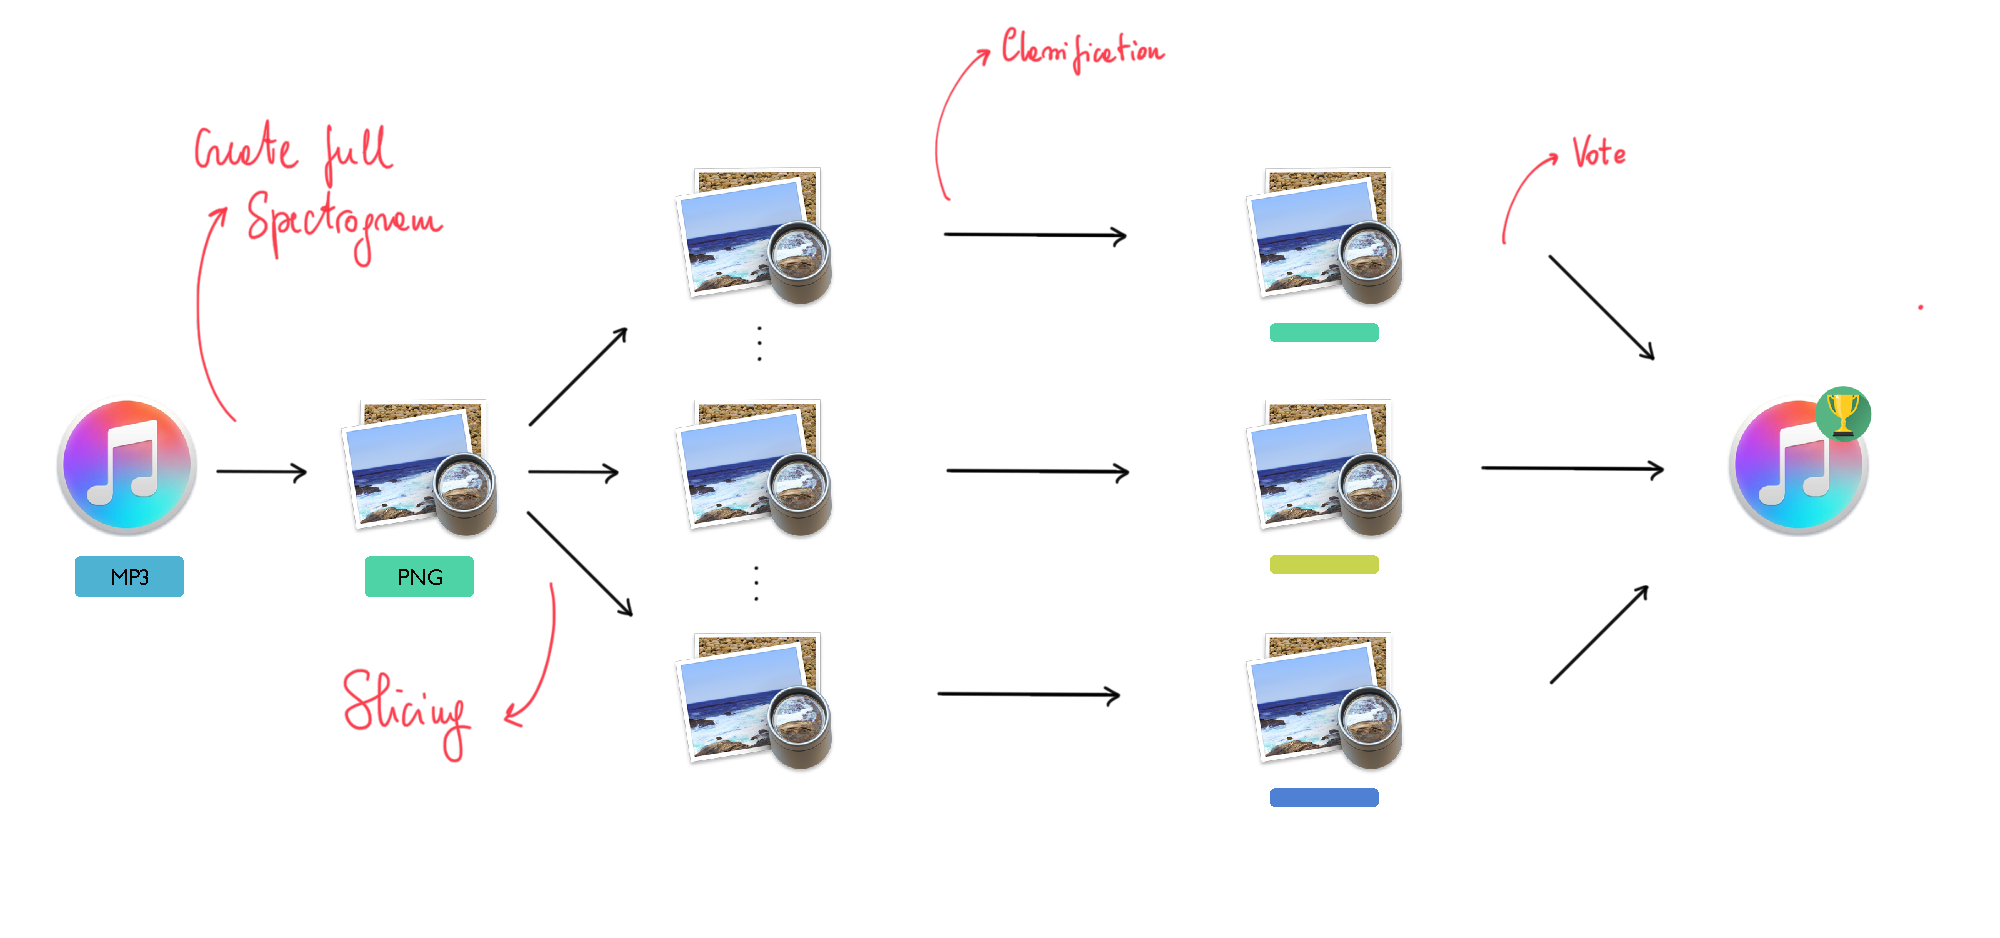
\includegraphics[width=0.8\linewidth]{img/Pipeline-project}
   \end{center}
      \caption{Classification pipeline.}
   \label{fig:pipeline}
   \end{figure*}



\section{Data preparation}\label{data-preparation}

\subsection{Training dataset}

The RAVDESS Emotional song audio consists of 1012 files of actors singing in a neutral North American accent. The portion used for this work includes calm, happy, sad, angry, and fearful emotions, each vocal is produced at two levels of emotional intensity, normal and strong.

Files are provided as .wav (16bit, 48kHz, mono, 4 seconds each) that need to be converted into raw spectrograms. For the purpose "SoX (Sound eXchange) sound processing utilities" has been used. This tool can process audio files and do things like trimming or filters frequencies. Spectrograms for the training dataset have been generated to fit the input size of the three networks, furthermore, to cope with the limited size of the dataset, augmentation has been applied like random grey colorizing, brightness, contrast and hue variations. Amiriparian \etal \cite{Amiriparian} showed that using different shades of colour could exhibit different outcomes. Unfortunately, since the hue transformation made by the PyTorch framework has a not negligible impact on the brightness of the image and the goal is to not corrupt the information brought by the spectrograms, the best choice was to stick with the original shades (Figure \ref{fig:training-sample}). Hence, playing with the contrast and with monochromes image could have a positive effect on capturing some features.

\begin{figure}[ht]
   \begin{center}
   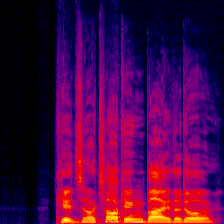
\includegraphics[width=0.8\linewidth]{img/happy_92.png}
   \end{center}
      \caption{Training spectrogram sample.}
   \label{fig:training-sample}
   \end{figure}

   \begin{figure*}
      \begin{center}
      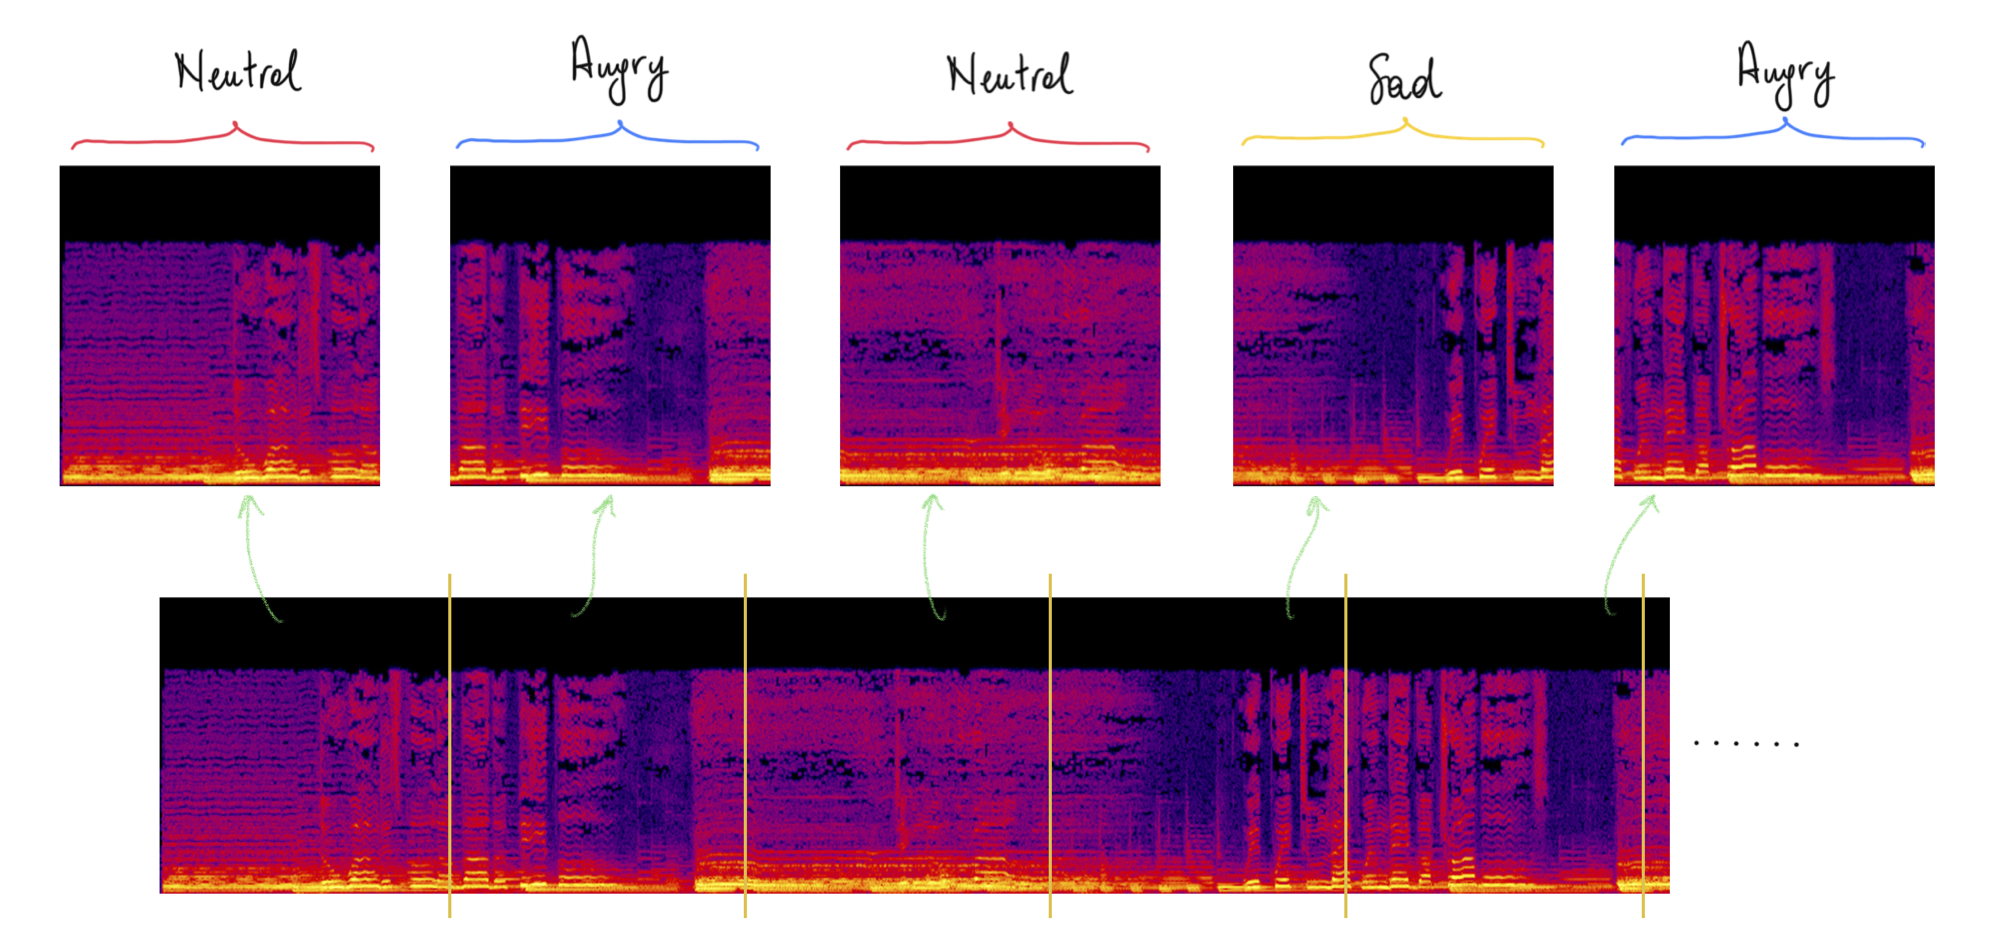
\includegraphics[width=0.8\linewidth]{img/voting-system}
      \end{center}
         \caption{Voting system.}
      \label{fig:voting}
      \end{figure*}

\subsection{Test dataset}\label{test-dataset}

The CAL500 dataset contains 500 songs performed by 500 unique artists, each song has been annotated by at least three people using a standard survey. Files are provided as .mp3 (32kbps, mono) along with one or more labels.

As Liu \etal \cite{Liu} stated \textit{preprocessing the spectrograms is a key point of successfully applying CNN on music spectrograms}, because the input to CNN requires to be a fixed size matrix and each track has a variable duration. The point is to let the network be able to recognize the emotion by taking a closer look at the song. The simplest approach would have been to extract spectrograms of the desired size after computing the number of overlaps. Yet, the chosen approach has been to not loose any data during the pre-processing step, thus the need is to define an algorithm that will generate spectrograms with variable length in order to match them to the duration of the tracks.
For the purpose of making the dataset compatible with our testing environment, two actions have been performed.

\subsubsection{Filtering}\label{filtering}

Since the training label set was a subset of the CAL500 labels, we selected only the songs which classes belong to the first set. Furthermore, an additional filtering step has been performed to remove all the redundant classes keeping only the relevant ones.

\subsubsection{Slicing}

The most challenging step was making the test dataset compatible with the training samples. To cope with the variable duration of each song, the extracted spectrograms have been sliced into squared images to fit to the network input size without losing any information. Each slice has been generated by sampling a proportional quantity of information equal to the training samples of four seconds. In fact, SoX allows to extract the spectrogram by setting the number of pixel per second and the input size of the image. Given that, a different testing approach has been implemented.

\section{Training phase}\label{training}

The research method to find the optimal set of hyperparameters has been the same for all networks\footnote {ResNet50 \& ResNet152, VGG11 \& VGG19 and GoogLeNet (Inception v1)} except for a slight difference related to GoogLeNet due to its three output branches. A lot of experiments have been done on different network variants of the same model to evaluate the impact of the networks' depth on the results.

The first step was to find a good starting hyperparameters set to make the network accomplish a full training. Due to Google Colab limitations, a random search has been used to evaluate 50 different hyperparameters sets. The approximate best ones have been reported in Table \ref{tab:sets}.

\begin{table}
   \begin{center}
      \def\arraystretch{1.5}
   \begin{tabular}{l|c|c|c|c}
   \textbf{Network} & \textbf{LR} & \textbf{BS} & \textbf{WD} & \textbf{G} \\
   \hline
   ResNet152 & 0.003 & 12 & 2e-05 & 0.6 \\
   \hline
   ResNet50 & 0.0007 & 14 & 8e-04 & 0.7 \\
   \hline
   VGG19 & 0.003 & 8 & 3e-04 & 0.01 \\
   \hline
   VGG11 & 0.0005 & 8 & 3e-05 & 0.05 \\
   \hline
   GoogLeNet & 0.0001 & 8 & 5e-05 & 0.1 \\
   \end{tabular}
   \end{center}
   \caption{Best values per hyperparameter.}
   \label{tab:sets}
   \end{table}



Using the reported sets, all the networks have been trained for 100 epochs and evaluated using different split ratios between training set and validation set. The final values have been selected by doing some tuning by hand after evaluating the networks' performance during the epochs, moreover the values of each hyperparameter have been adjusted to address the problem of the high epochs number and to prevent the occurring overfit. Since the training dataset is very small, we dealt with the overfit problem by means of data augmentation, yet no significant improving has been noticed.

Table \ref{tab:val} contains the average best validation scores calculated on the validation set per network and variants. Due to lack of time, different combinations of criterions and optimizers have not been tested. However we observed that choosing a validation set of a smaller size, the overall score of all networks will increase. Although the training dataset is small, applying a significative amount of regularization prevented the occurring of the overfitting phenomenon seen right after half of the epochs, but the limitations imposed by the platform kept us from increasing the number of epochs and evaluating more sets of hyperparameters.

\begin{table}[ht]
   \begin{center}
   \def\arraystretch{1.5}
   \begin{tabular}{l|c|c|c}
      \textbf{Network} & \textbf{50/50} & \textbf{80/20} & \textbf{90/10} \\
   \hline
   \textit{ResNet152} & \% & 56\% & 76\% \\
   \hline
   \textit{ResNet50} & \% & 62\% & \% \\
   \hline
   \textit{VGG19} & \% & 61\% & \% \\
   \hline
   \textit{VGG11} & \% & 65\% & \% \\
   \hline
   \textit{GoogLeNet} & 72\% & 73\% & 82\% \\
   \end{tabular}
   \end{center}
   \caption{Average validation accuracy per network and split in 100 epochs.}
   \label{tab:val}
   \end{table}

\section{Testing}\label{testing}

The testing phase was characterized by two main parts: the network slices' prediction and the major voting.
During the first part, the network assigned a prediction to each slice. The PyTorch \textit{DataLoader} class, used in this part to collect a batch of images to be classified, was modified with the intention to have the image path as another return value, together with the image tensor and its labels. In this way it was possible to collect, for each song, a set of counters, one for each possible test class increased each time a prediction for a specific class was done.

In the second part all the data collected in the previous one were processed in order to decide which class was more predicted by the model, for each song, using a pure major voting strategy: the higher counter labeled the entire song. A preprocessing step for this part on the test dataset's labels was useful. In fact, for getting this values in an immediate way, a mapping on all songs was previously done, assigning for each song all the labels belonging to the subset obtained in Section \ref{filtering}.

Processing the data collected in network prediction's part, a dominant label was assigned to each song. A song is correctly classified if the predicted label was in the subset of the attributed labels. Finally, with the number of correct predictions and the total number of songs considered in the test dataset, it was possible to calculate the test accuracy.



   \begin{table}[ht]
      \begin{center}
      \def\arraystretch{1.5}
      \begin{tabular}{l|c|c|c}
         \textbf{Network} & \textbf{50/50} & \textbf{80/20} & \textbf{90/10} \\
      \hline
      \textit{ResNet152} & \% & \% & 35\% \\
      \hline
      \textit{ResNet50} & \% & \% & \% \\
      \hline
      \textit{VGG19} & \% & \% & \% \\
      \hline
      \textit{VGG11} & \% & \% & \% \\
      \hline
      \textit{GoogLeNet} & 36\% & 34\% & 37\% \\
      \end{tabular}
      \end{center}
      \caption{Test accuracy per network and split.}
      \label{tab:test}
      \end{table}

      \begin{figure}[ht]
         \begin{center}
         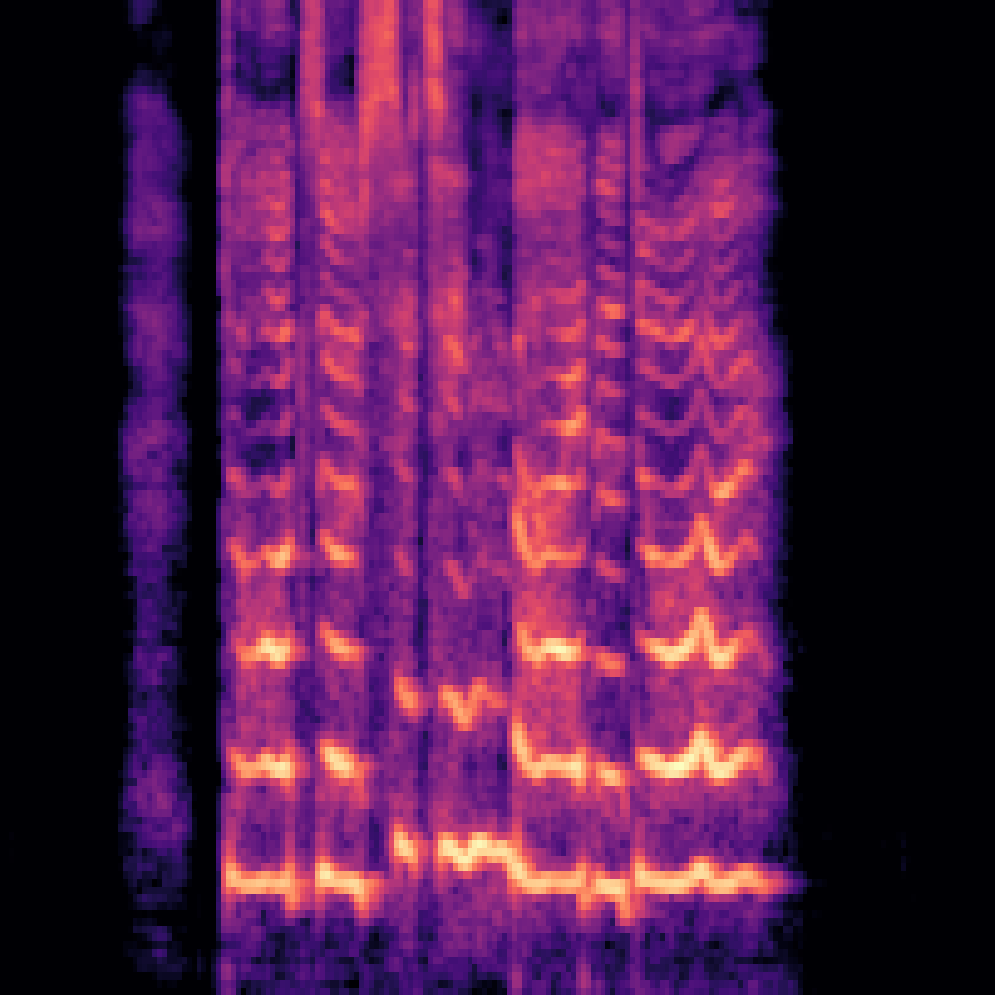
\includegraphics[width=0.8\linewidth]{img/mel-spectrogram.png}
         \end{center}
            \caption{Mel spectrogram sample from the training set.}
         \label{fig:mel-sample}
         \end{figure}

\section{Conclusions}\label{conclusions}

This report proposed an experimental method to classify songs with emotions captured from human vocal singing recordings.

Since the networks extracted features from spectrograms related to pure vocals, we had many doubts that the correct classification of spectrograms related to songs (vocal and instrumental) would be taken for granted. The accuracies' values suggest us that our doubts were real. Hence, the first immediate suggestion to achieve the right classification is to find emotions within a single domain. To stay in our domain (vocal), we should have extracted only the voice channel from each song, removing the instrumental part. Such process cannot be achieved within an acceptable time span. The biggest problem was the lack of availability of bigger and free datasets for this task.

This being cleared up, we can now suggest further improvements.

The use of mel spectograms (Figure \ref{fig:mel-sample}) could have resulted in better performances as found out also by Eguino \cite{Eguino}. After a couple of validation runs, each network performed a lot better than training on raw spectrograms, actually, networks like VGG19 reached very high validation scores (94\% using a 80/20 split). The preprocessing steps, unfortunately, required additional libraries like \textit{librosa} that are not trivial to use for extracting variable spectrograms like those described in Section \ref{test-dataset}.

The testing phase can be improved in different ways. One possibility is to change the major voting algorithm. An example can be: insert a threshold to define the most predicted label, considering the percentage of the specific prediction on all slices. In this way the cases in which the most important label is not so dominant are excluded. Another possibility is to change how the predictions are considered as correct: having a definition of test class rank importance can determine different levels of prediction rightness. The consequence is to define a new method for calculate the accuracy on the test dataset.

Future works could be based on these suggested improvements. Full code is available at \url{https://github.com/anphetamina/AIML_project}.

{\small
\bibliographystyle{ieee_fullname}
\bibliography{egbib}
}


\end{document}
